\begin{figure}[t]\centering
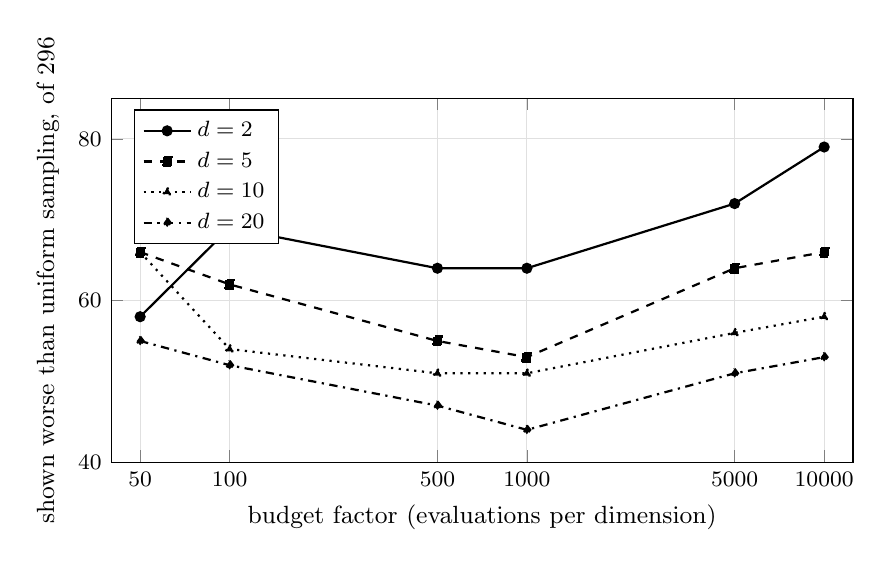
\begin{tikzpicture}
\begin{axis}[width=11cm,height=6.2cm,
  xmode=log,log basis x=10,
  xlabel={budget factor (evaluations per dimension)},
  ylabel={shown worse than uniform sampling, of 296},
  ymin=40,ymax=85,xmin=40,xmax=12500,
  xtick={50,100,500,1000,5000,10000},
  xticklabels={50,100,500,1000,5000,10000},
  legend pos=north west,legend cell align=left,
  grid=major,grid style={black!12},
  tick label style={font=\footnotesize},label style={font=\small},
  legend style={font=\footnotesize}]
\addplot[thick,mark=*,mark size=1.6pt] coordinates
  {(50,58)(100,69)(500,64)(1000,64)(5000,72)(10000,79)};
\addlegendentry{$d=2$}
\addplot[thick,mark=square*,mark size=1.6pt,dashed] coordinates
  {(50,66)(100,62)(500,55)(1000,53)(5000,64)(10000,66)};
\addlegendentry{$d=5$}
\addplot[thick,mark=triangle*,mark size=1.6pt,dotted] coordinates
  {(50,66)(100,54)(500,51)(1000,51)(5000,56)(10000,58)};
\addlegendentry{$d=10$}
\addplot[thick,mark=diamond*,mark size=1.6pt,dashdotted] coordinates
  {(50,55)(100,52)(500,47)(1000,44)(5000,51)(10000,53)};
\addlegendentry{$d=20$}
\end{axis}
\end{tikzpicture}
\caption{Implementations shown strictly worse than uniform sampling at equal budget,
of 296, exact sign test with Holm at 5\% per (dimension, budget). The count rises
toward the top budget in every dimension, from a mid-grid minimum in 5, 10 and 20
dimensions: a search that stalls is overtaken by a control that keeps sampling.}
\label{fig:trend}
\end{figure}
